\section{Ejercicio 8}
En la naturaleza la informaci\'on est\'a siempe caracterizada por señales anal\'ogicas. Con el fin de manipular e interpretar dichas señales mediante un procesador o algun tipo de circuto l\'ogico es necesario convertir las señales anal\'ogicas (continuas en el tiempo) a señales digitales (discretas en el tiempo). Un conversor anal\'ogico digital (ADC por sus sigas en ingl\'es), cumple la funci\'on de digitaizar señales continuas en el tiempo. Se manejan dos par\'ametros en la conversi\'on de señales: el Sampling Rate ($f_s$) y el Sampling Precision ($N$). El primero representa la cantidad de muestras que se toman por segundo, mientras que el segundo par\'ametro define la cuantizaci\'on en amplitud de la señal. En el caso ideal tanto el Sampling Rate como el Sampling Precsion deber\'ian ser infinitos y as\'i se obtendr\'ia la señ al original. Sin embargo, ni existe memoria suficiente para almacenar una cantidad infinita de puntos ni ser\'ia pr\'actico su almaceamiento. En el caso de estudio la señal que debe digitalizarse es la salida de un potenci\'ometro presente en un Joystick anal\'ogico. Con ese fin se decidió separar el diseño en varios bloques que cumplieran tareas específicas, facilitando entre otras la implementación y el testo. Los bloques utilizados fueron un generador de rampa, un comparador, un generador de clock y un contador. Su propuesta de diseño e implementación se presentan a continuación. \par


%%%Agregar diagrama de boques con partes del diseño.

\subsection{Diseño}

\subsubsection{Generador de Rampa}

Primeramente, se necesitó medir de cierta manera la variación en la tensión provista por el joystick, la cual será proporcional a su posición respecto del eje. Esto se debe a que internamente el joystick cuenta con un ponteciómetro que provee entre $0\,V$ y $5\,V$. Por ende, se diseñó una rampa utilizando un circuito integrado $NE555$, la misma se utilizará para comparar tensiones. \par

\begin{figure}[H]
\centering
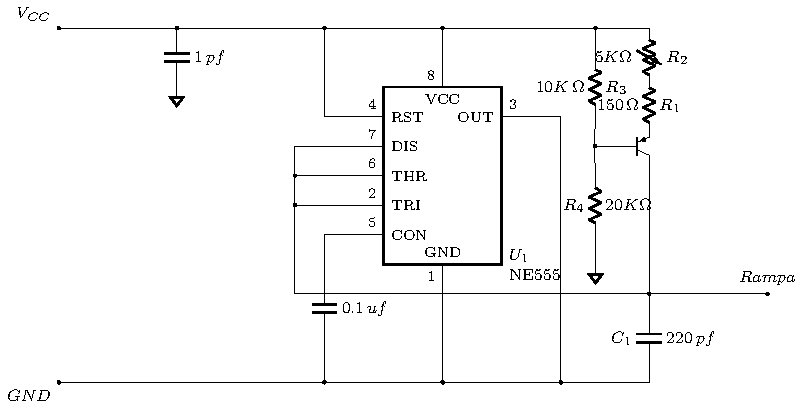
\includegraphics[scale=0.8]{Ejercicio8/Circuitos/Generador_de_rampa.pdf}
\caption{Generador de Rampa con desfasaje}
\label{fig:Generador_de_rampa}
\end{figure}

La rampa representará la carga del capacitor $C_1$ presente en el circuito (\ref{fig:Generador_de_rampa}), dicha carga será constante debido a que el componente anteriormente mencionado está conectado con el colector del transistor PNP que está actuando como fuente de corriente. La tasa de refresco estará dada por la frecuencia de la rampa, debido a que la cátedra solicitó una tasa de entre 1 y 20 segundos, fue necesario añadir componentes variables al circuito. Para lograr dicha variación, se cambiará la pendiente de la misma, dada por $S=\frac{I_C}{C_1}$. Para comenzar, se decidió fijar el valor de $C_1$ en $220\,pf$ tal que sólo sea variable $I_C$. Por otro lado, la corriente en el colector está dada por:

\begin{equation}
I_C=\frac{V_{CC}-V_E}{R_E}
\end{equation}

La tensión en el emisor está determinada por un divisor resistivo dado por:

\begin{equation}
V_E=\frac{R_4}{R_4+R_3} * V_{CC} + V_{BE}
\end{equation}

Se fijaron los valores de $R_4$ y $R_3$ en $20K\,\Omega$ y $10K\,\Omega$ respectivamente, tal que la única incógnita sea $R_E$. \par
Para obtener una tasa de refresco de entre 1 y 20 segundos se necesitará que $R_E$ varíe entre $150\,\Omega$ y $4K\,\Omega$. Consecuentemente, se pondrán dos resistencias en serie, siendo la primer resistencia($R_1$), fija con valor nominal $150\,\Omega$ mientras que la segunda($R_2$) será un potenciómetro de $5K\,\Omega$.

Como primer problema a solucionar para el diseño, surgió que la pendiente de la rampa se encontraba entre $5\,V$ y $10\,V$ como se puede ver en la imagen (\ref{fig:Generador_de_rampa_LTSpice}). Esto se debía a la construcción propia del N555 que utiliza comparadores para obtener una señal de salida entre un tercio y dos tercios de la tensión de alimentación ($V_{CC}$), en nuestro caso, $15\,V$.


\begin{figure}[H]
\centering
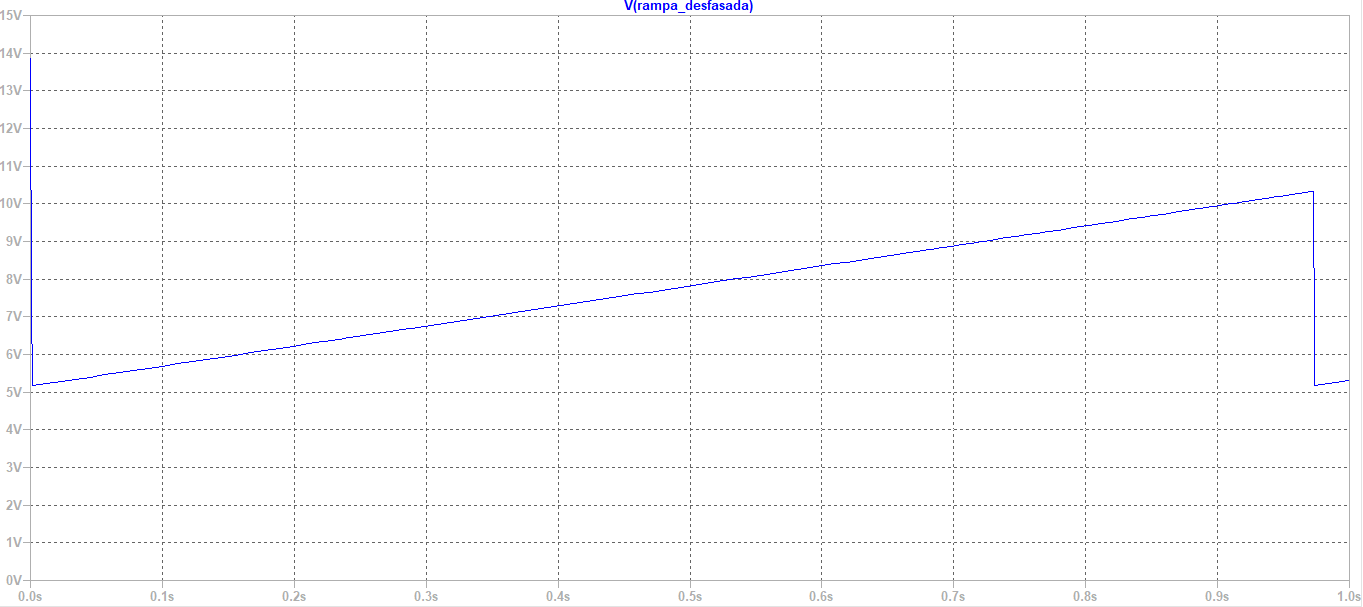
\includegraphics[width=0.7\textwidth]{Ejercicio8/Imagenes/Rampa_desfasada}
\caption{Tensión de la rampa con desfasaje}
\label{fig:Generador_de_rampa_desfasada_LTSpice}
\end{figure}

Por ende, se implementó un amplificador operacional que funcionará como restador para reducir la tensión de salida de la rampa en $5\,V$, utilizando el siguiente circuito:

\begin{figure}[H]
\centering
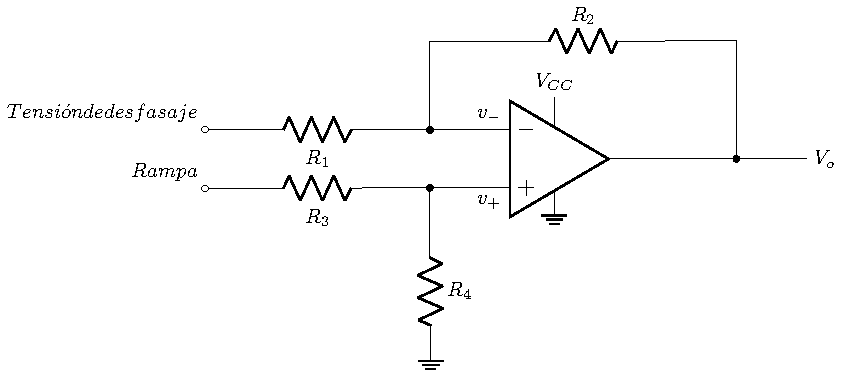
\includegraphics[scale=0.8]{Ejercicio8/Circuitos/Restador.pdf}
\caption{Restador}
\label{fig:Restador}
\end{figure}
La salida del amplificador operacional va a estar dada por:
\begin{equation}
V_o=\frac{-R_2}{R_1}V_2+\left(1+\frac{R_4}{R_3}\right)V_1
\end{equation}
Tomando valores de resistencias equivalentes, obtendremos:
\begin{equation}
V_o=-V_2+V_1
\end{equation}
Siendo $V_1$ la tensión de la rampa y $V_2$ la tensión de desfasaje.\par\par
Se obtuvo la siguiente rampa acorde a las necesidades para el trabajo:

\begin{figure}[H]
\centering
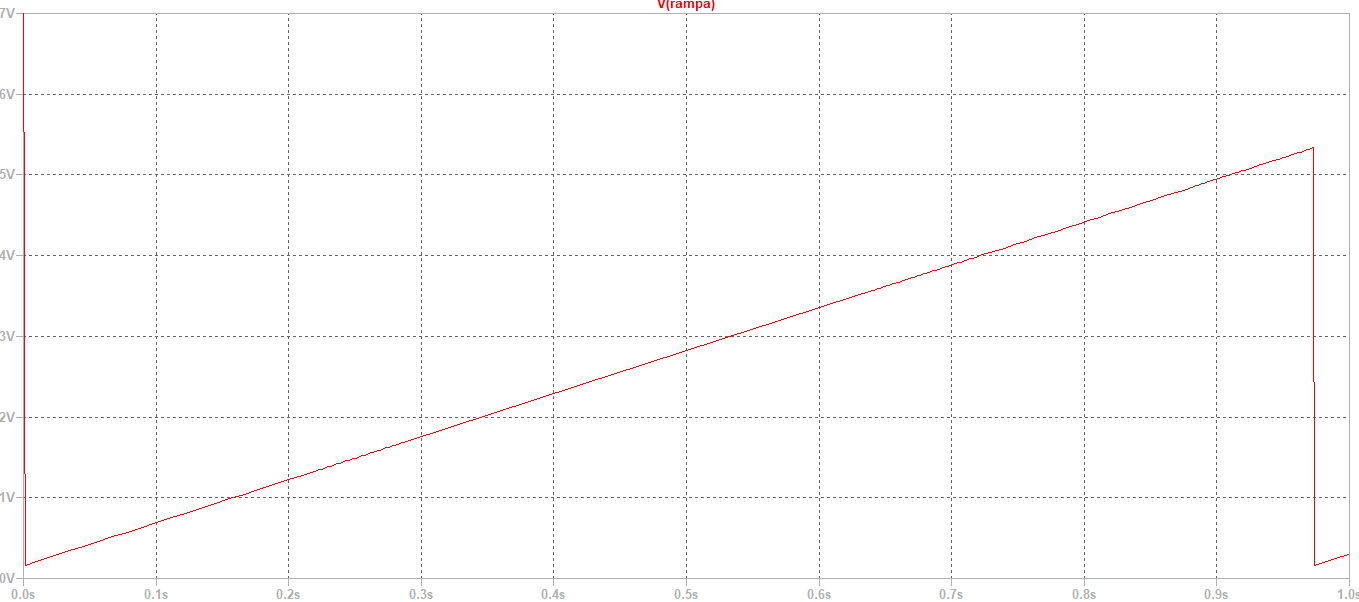
\includegraphics[width=0.7\textwidth]{Ejercicio8/Imagenes/Rampa}
\caption{Tensión de la rampa}
\label{fig:Generador_de_rampa_LTSpice}
\end{figure}



Se considera necesario aclarar la utilización de un buffer entre la salida de la rampa desfasada y el restador para que no se modifiquen los comportamientos entre ambos circuitos.\par

\subsubsection{Clock}


\subsubsection{Comparador}

\begin{figure}[H]
\centering
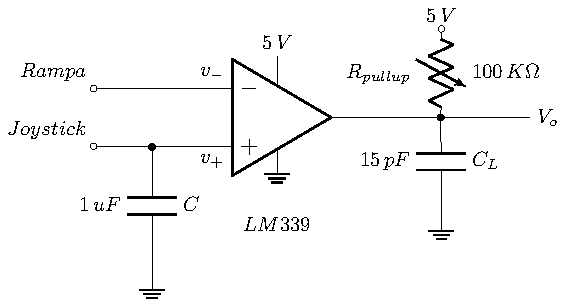
\includegraphics[scale=0.8]{Ejercicio8/Circuitos/Comparador.pdf}
\caption{Comparador de tensiones}
\label{fig:Comparador}
\end{figure}

\subsubsection{Contador}

\begin{figure}[H]
\centering
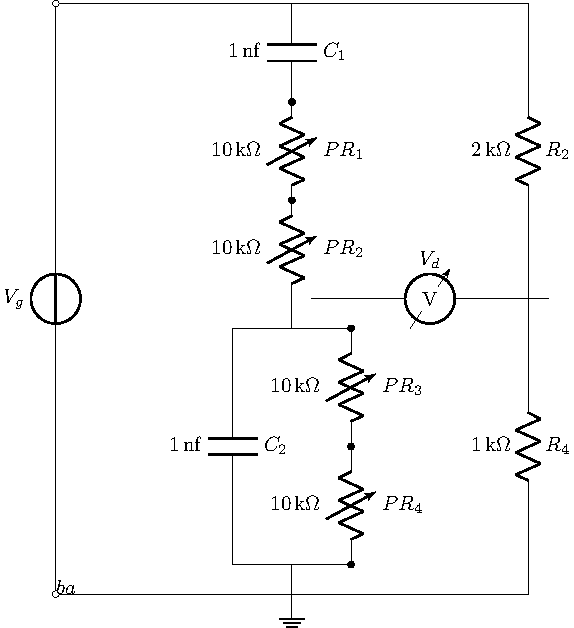
\includegraphics[scale=0.8]{Ejercicio8/Circuitos/Contador&Display.pdf}
\caption{Contador}
\label{fig:Contador&Display}
\end{figure}

\begin{figure}[H]
\centering
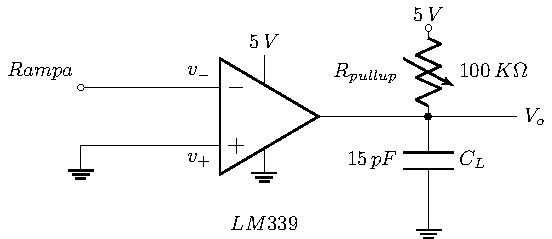
\includegraphics[scale=0.8]{Ejercicio8/Circuitos/Reset.pdf}
\caption{Reset}
\label{fig:Reset}
\end{figure}





\subsection{Conclusiones}